\section{Processes of the Central Dogma}
Up to this point, we have considered a variety of transport and biosynthetic
processes that are critical to acquiring and generating new cell mass. We now
turn our focus to some of the most important processes which \textit{must} be
undertaken irrespective of the growth conditions -- those of the central dogma.

To successfully divide and produce viable progeny, the DNA must be faithfully
replicated and segregated into each nascent cell. In rapidly growing cultures,
bacteria like \textit{E. coli} can initiate as many as 10 - 12 replication forks
at a given time \citep{bremer2008, si2017}, suggesting  only $\approx 10$ are
needed. However, as shown in \FIG{central_dogma}(A), DNA polymerase III is
nearly an order of magnitude more abundant while still maintaining a predicted
growth rate dependence. This discrepancy can be understood by considering its
binding constant to DNA. \textit{In vitro} characterization has quantified the
$K_D$ of DNA polymerase III holoenzyme to single-stranded and double-stranded
DNA to be 50 and 200 nM, respectively \citep{ason2000} \FIG{central_dogma}(B)
(discussed further, along with the synthesis of dNTP building blocks in Appendix
Section "Additional Process of the Central Dogma").

\begin{figure}
    \centering{
    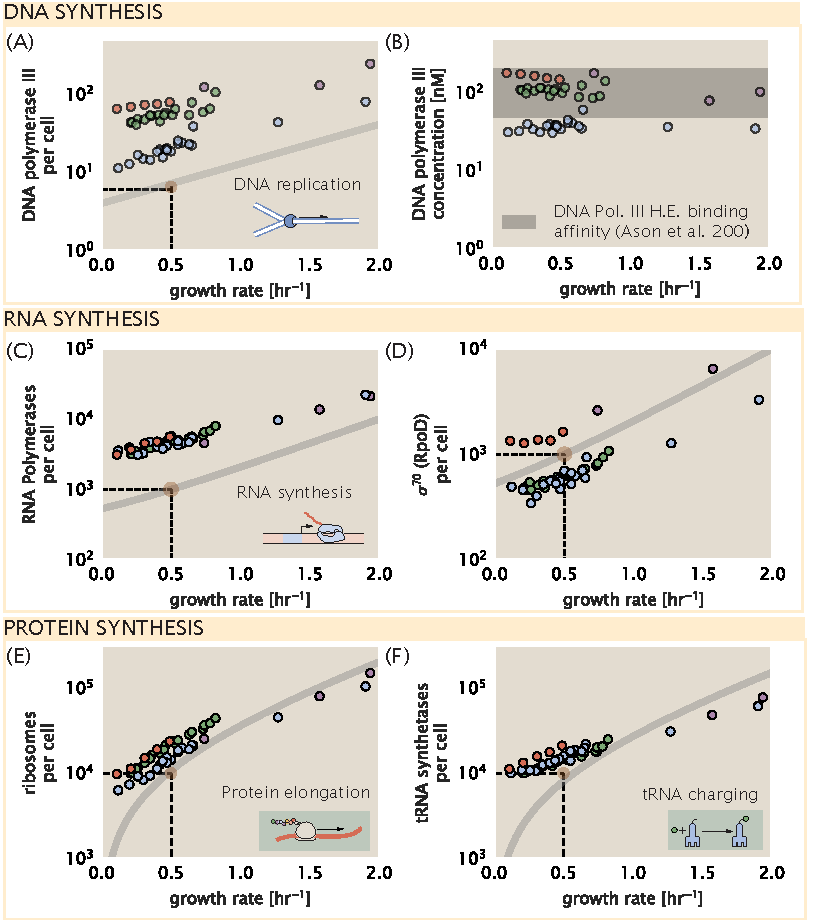
\includegraphics[width=0.55\textwidth]{main_figs/fig4_central_dogma.pdf}
    \caption{\textbf{Processes of the central dogma.}
    (A) The minimum number of DNA polymerase holoenzyme complexes needed to
        facilitate replication of the genome. Points correspond
        to the total number of DNA polymerase III holoenzyme complexes
        ([DnaE]$_3$[DnaQ]$_3$[HolE]$_3$[DnaX]$_5$[HolB][HolA][DnaN]$_4$[HolC]$_4$[HolD]$_4$)
        per cell.
    (B) The effective concentration of DNA polymerase III
        holoenzyme (See Appendix Section "Estimation of Cell Size and Surface Area" for calculation of cell
        size). Shaded region corresponds to the range of $K_D$ values measured by \cite{ason2000},
        from 50 and 200 nM.
    (C) The number of RNA polymerase core enzymes, with measurements corresponding
        to the average number given a subunit stoichiometry of
        [RpoA]$_2$[RpoC][RpoB].
    (D) The abundance of $\sigma^{70}$ as a function of growth rate along with the same
        prediction from (C).
    (E) Number of ribosomes required to synthesize 10$^9$ peptide bonds with an
        elongation rate of 15 peptide bonds per second.
    (F) Number of tRNA synthetases that
        will supply the required amino acid demand. The sum of all tRNA
        synthetases copy numbers are plotted
        ([ArgS], [CysS], [GlnS], [GltX], [IleS], [LeuS], [ValS], [AlaS]$_2$,
        [AsnS]$_2$, [AspS]$_2$, [TyrS]$_2$, [TrpS]$_2$, [ThrS]$_2$,
        [SerS]$_2$, [ProS]$_2$, [PheS]$_2$[PheT]$_2$, [MetG]$_2$,
        [lysS]$_2$, [HisS]$_2$, [GlyS]$_2$[GlyQ]$_2$).
        Dashed lines indicate order of magnitude estimate needed at a
        growth rate of $\approx 0.5 $ per hr (light-brown point), while the gray line
        accounts for the growth rate dependence changes in cell size and doubling time.
    }
    \label{fig:central_dogma}
    }
\end{figure}


% \subsection{DNA Replication}
% To successfully divide and produce viable progeny, the DNA must be
% faithfully replicated and segregated into each nascent cell. Most bacteria
% (including \textit{E. coli}) harbor a single, circular chromosome and can have
% extra-chromosomal plasmids up to $\sim$ 100 kbp in length. We consider the
% supply of the dNTP building blocks in Appendix Section "Additional Process of
% the Central Dogma". Replication is initiated at a single region of the
% chromosome termed the \textit{oriC} locus where a pair of replisomes, each
% consisting of two DNA polymerase III, begin their high-fidelity replication of
% the genome in opposite directions \citep{fijalkowska2012}. \textit{In vitro}
% measurements have shown that DNA Polymerase III copies DNA at a rate of $\approx
% 600$ nucleotides per second (BNID: 104120). To replicate a single chromosome of
% $\approx 5\times 10^6$ base pairs, two replisomes moving at their maximal rate
% would copy the entire genome in $\approx$ 4000 s; well within out division time
% of 5000 seconds.


% In rapidly growing cultures, bacteria like \textit{E. coli} can initiate as many
% as 10 - 12 replication forks at a given time \citep{bremer2008, si2017},
% suggesting  only $\approx 10$ are needed. However, as shown in
% \FIG{central_dogma}(A), DNA polymerase III is nearly an order of magnitude more
% abundant but still maintains the expected growth rate dependence. This
% discrepancy can be  understood by considering its binding constant to DNA.
% \textit{In vitro} characterization has quantified the $K_D$ of DNA polymerase
% III holoenzyme to single-stranded and double-stranded DNA to be 50 and 200 nM,
% respectively \citep{ason2000}. The concentration of DNA polymerase III across
% all data sets apear in this range and cells vary theircopy number such that its
% concentration is approximately equal to the dissociation constant to the DNA.
% While the processes regulating the initiation of DNA replication are complex and
% involve more than just the holoenzyme, these data indicate that the kinetics of
% replication rather than the explicit copy number of the DNA polymerase III
% holoenzyme is the more relevant feature of DNA replication to consider. In light
% of this, DNA replication does not represent a rate-limiting step in
% cell division. Interestingly, it is worth noting that for bacterium like \textit{C.
% crescentus} whose chromosomal replication is initiated only once per cell cycle
% \citep{jensen2001}, the time to double their chromosome indeed represents an
% upper limit to their growth rate.
